\documentclass[addpoints,12pt]{exam}

\usepackage{fullpage}
\usepackage{amsmath}
\usepackage{amssymb}
\usepackage{amsfonts}
\usepackage{amsthm}
\usepackage{textcomp}
\usepackage{color}
\usepackage{enumerate}
\usepackage{pdfpages}
\usepackage{pgfplots}
\usepackage{wrapfig}
\usepackage{enumitem}
\usepackage{bm}
\usepackage{graphicx}
\usepackage[font=small]{caption}
\usepackage{tikz}
\usepackage{tcolorbox}
\usepackage[thinc]{esdiff}


\newcommand{\ZZ}{\mathbb{Z}}
\newcommand{\RR}{\mathbb{R}}
\newcommand{\QQ}{\mathbb{Q}}
\newcommand{\NN}{\mathbb{N}}
\newcommand{\CC}{\mathbb{C}}
\newcommand{\PP}{\mathbb{P}}
\newcommand{\x}{\times}
\newcommand{\rto}{\xrightarrow}
\newcommand{\lto}{\lrightarrow}
\newcommand{\tbf}{\textbf}

\pagestyle{headandfoot}
\usepackage{lmodern}
\usepackage[T1]{fontenc}
\definecolor{coral}{RGB}{255,127,80}

\begin{document}

\firstpageheader{CSE 176 Assignment 1}{ }{\makebox[0 in]{Fall 2024}}
\noindent Due at \textbf{11:59PM Wednesday October 9, 2024} \\
Total points: \textbf{10 points} which is 10\% of course grade.
\\
\noindent What to submit: Put your answers in solution sections bellow and submit a PDF to CatCourses. Select all choices that apply for multiple-choices problems.

\noindent What to edit: Edit the provided .tex. It is recommended to use overleaf and clone the project (https://www.overleaf.com/read/vfhqsvqkwgyv\#107642).\\

\noindent Student Name:
\runningheadrule
\runningheader{Assignment 1}{}{Page \thepage\ of \numpages}

\begin{center}
\makebox[\textwidth]{\enspace\hrulefill}\\ 
\end{center}

\noindent\textbf{{\large Part I: Linear Algebra and Probability}}


\begin{questions}



\question[1] Which of the following vectors are in the span of the vectors {\begin{bmatrix} 1 \\ 2 \\ -1 \end{bmatrix}},{\begin{bmatrix} 3 \\ 1 \\ 2 \end{bmatrix}}? 
\begin{enumerate}[label=(\alph*)]
\item \begin{bmatrix} 5 \\ 5 \\ 0 \end{bmatrix}
\item \begin{bmatrix} 0 \\ 0 \\ 1 \end{bmatrix}
\item \begin{bmatrix} -1 \\ 0 \\ 1 \end{bmatrix}
\item \begin{bmatrix} 7 \\ -1 \\ 8 \end{bmatrix}
\end{enumerate}

\textbf{\textit{{\color{coral} Solution:}}}


\question[1] Let \[A=\begin{bmatrix}2 & 0 & 1 \\ 3 & 0 & -2 \end{bmatrix},B=\begin{bmatrix}2 & 2 & 1 \\ 0 & 1 & 1 \end{bmatrix},\]

Find the inverse of $AB^T$.

\textbf{\textit{{\color{coral} Solution:}}}

%\[(AB^T)^{-1}=\begin{bmatrix}0.2 & 0  \\ -0.6 & 0.5  \end{bmatrix}\]

\question[1] Which of the following statement is always true?
\begin{enumerate}[label=(\alph*)]
\item If $A$ is a 3×5 matrix and $B$ is a 5×4 matrix, then $(AB)^T$ is a 3×4 matrix.
\item If $A=A^T$, then the diagonal entries of $A$ must be either 0 or 1’s.
\item If $AB=A^TB^T$, then $A$ and $B$ must be of the same size.
\item $AA^T=A^TA$
\end{enumerate}

\textbf{\textit{{\color{coral} Solution:}}}


\question[1] A random variable, $X$, has the probability distribution table as shown.

\begin{table}[h]
\begin{tabular}{|l|l|l|l|l|l|}
\hline
\textit{}  x & 0 & 1 & 2 & 3 & 4 \\ \hline
         $P(X=x)$ &  &  & 0.2 & 0.3 & 0.3 \\ \hline
\end{tabular}
\end{table}

Assume that $P(X=0)=P(X=1)$). Compute the expectation and variance of $X$. 

\textbf{\textit{{\color{coral} Solution:}}}

\hspace{-0.25in}\noindent\textbf{{\large Part II: Supervised Learning and Classification}}

\question[1] Which of the following corresponds to underfitting?

\begin{enumerate}[label=(\alph*)]
\item High training error, low testing error
\item High training error, high testing error
\item Low training error, high testing error
\item Low training error, low testing error
\end{enumerate}

%\question Explain in a few sentences why a validation set is needed sometimes besides training and testing set for machine learning problems.

\textbf{\textit{{\color{coral} Solution:}}}


\hspace{-0.25in}\noindent\textbf{{\large Part III: Clustering}}

\question[1] Which of the following is true about Lloyd’s algorithm for k-means clustering?

\begin{enumerate}[label=(\alph*)]
\item It is a supervised learning algorithm.
\item If run for long enough, it will always terminate.
\item It can give a nonlinear boundary between two clusters.
\item It can give global optimal solution.
\end{enumerate}

\textbf{\textit{{\color{coral} Solution:}}}

\question 
\begin{parts}

\part[1] Write the mean and median vector for the following set of 2D points. If there are multiple mean or median vectors, write only one such vector.

$x_1$ = $\begin{bmatrix} 5 \\ 5  \end{bmatrix}$, 
$x_2$ = $\begin{bmatrix} 3 \\ 0  \end{bmatrix}$,
$x_3$ = $\begin{bmatrix} -2 \\ 9  \end{bmatrix}$,
$x_4$ = $\begin{bmatrix} 6 \\ 2  \end{bmatrix}$,
$x_5$ = $\begin{bmatrix} 7 \\ -5  \end{bmatrix}$

\textbf{\textit{{\color{coral} Solution:}}} 


\part[1] What is the advantage of K-medians clustering v.s. K-means clustering? Explain in a few sentences.

\textbf{\textit{{\color{coral} Solution:}}} 

\end{parts}



\question[2] Consider the following graph for which we would like to apply normalized cut clustering,

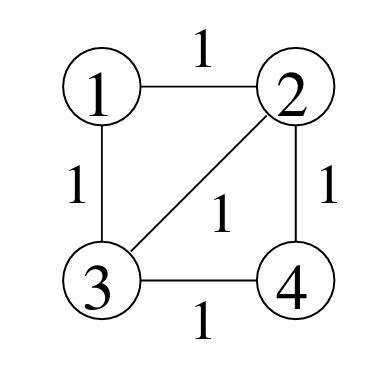
\includegraphics[width=.2\textwidth]{fig/graph.png}


\begin{parts}
\part[1] Write the affinity matrix $A$, degree matrix $D$, and Laplacian matrix $L=D-A$.

\textbf{\textit{{\color{coral} Solution:}}}

\part[1] What eigenproblem needs to be solved in normalized cut algorithm?

\textbf{\textit{{\color{coral} Solution:}}}

\end{parts}
\end{questions}
\end{document}
